\documentclass[11pt]{article}
\usepackage[a4paper,margin=1in]{geometry}
\usepackage{times}
\usepackage{graphicx}
\usepackage{booktabs}
\usepackage{amsmath,amssymb}
\usepackage{siunitx}
\usepackage{multirow}
\usepackage{hyperref}
\usepackage{xcolor}
\usepackage{float}
\usepackage{caption}
\usepackage{subcaption}
\usepackage{algorithm}
\usepackage{algpseudocode}
\usepackage{tikz}
\usetikzlibrary{arrows.meta,positioning,shapes.geometric}

\title{Effect of Data Preprocessing on Machine Learning Models:\\
A Corruption Diagnosis and Hardening Pipeline for Satellite Imagery}
\author{Aryan Arvind et al.\\
Department of Computer Science\\
Your Institute Name}
\date{\today}

\newcommand{\maybegraphic}[3]{%
\IfFileExists{#1}{\includegraphics[#2]{#1}}{%
\fbox{\parbox[c][0.30\textheight][c]{0.9\linewidth}{\centering Missing file: #1\\Upload this figure to Overleaf}}%
}%
}

\begin{document}
\maketitle

\begin{abstract}
Preprocessing failures in remote sensing pipelines can significantly degrade downstream model performance, yet most vision benchmarks assume clean and correctly preprocessed inputs. This paper presents an end-to-end implementation that explicitly models realistic preprocessing failures, diagnoses failure type and severity, restores corrupted inputs, and quantifies downstream impact using object detection behavior. The framework contains three main deep-learning components: (i) a physically grounded corruption injector that simulates six preprocessing failure families at three severity levels, (ii) a multi-task diagnosis convolutional neural network (CNN) for failure type and severity prediction, and (iii) a hardening autoencoder with a Kick-style decoder for image restoration. We evaluate the system on EuroSAT image data and measure diagnosis accuracy, restoration quality (PSNR, SSIM), and downstream detector stress/recovery trends. Results show that corruption effects are highly non-uniform across failure families and that recovery gains are corruption-dependent. The key contribution is a reproducible robustness analysis pipeline for studying preprocessing sensitivity, rather than a single-point clean-data accuracy claim.
\end{abstract}

\noindent\textbf{Keywords:} preprocessing robustness, satellite imagery, corruption diagnosis, image restoration, YOLOv8, deep learning pipeline

\section{Introduction}
Machine learning models in remote sensing often operate under an implicit assumption: upstream preprocessing is correct. In practice, this assumption fails due to atmospheric artifacts, compression, sensor noise, calibration drift, and cross-band misalignment. Such failures can silently change model behavior even when architecture and weights remain unchanged.

This work studies the \emph{effect of preprocessing quality} on downstream machine learning behavior through a full implementation pipeline. Instead of treating corruption as random augmentation noise, we model physically motivated failure modes and track their impact through diagnosis, restoration, and downstream detection.

\textbf{Research questions.}
\begin{enumerate}
\item How strongly do different preprocessing failure modes degrade downstream model behavior?
\item Can a learned model diagnose failure type/severity reliably enough for analysis?
\item Can a learned hardening model recover part of the downstream loss?
\end{enumerate}

\textbf{Contributions.}
\begin{enumerate}
\item An executable corruption-diagnosis-hardening-evaluation pipeline for satellite imagery.
\item A multi-task diagnosis CNN for corruption type and severity prediction.
\item A restoration autoencoder with artifact-reduced Kick-style upsampling.
\item A stress-curve-based downstream evaluation protocol and reproducible artifacts.
\end{enumerate}

\section{Related Work}
YOLOv8 has shown strong utility for military object detection in satellite imagery, motivating detector-centric downstream evaluation in high-stakes scenarios \cite{prathyusha2025yolo}. Deep learning-based satellite restoration methods also demonstrate that learned reconstruction can recover useful structure under real sensor corruption \cite{sensors2022landsat}. Building on these directions, our work integrates corruption simulation, diagnosis, restoration, and detector stress testing into one reproducible pipeline.

\section{Methodology}
\subsection{System overview}
Figure~\ref{fig:flowchart} summarizes the complete framework.

\begin{figure}[H]
\centering
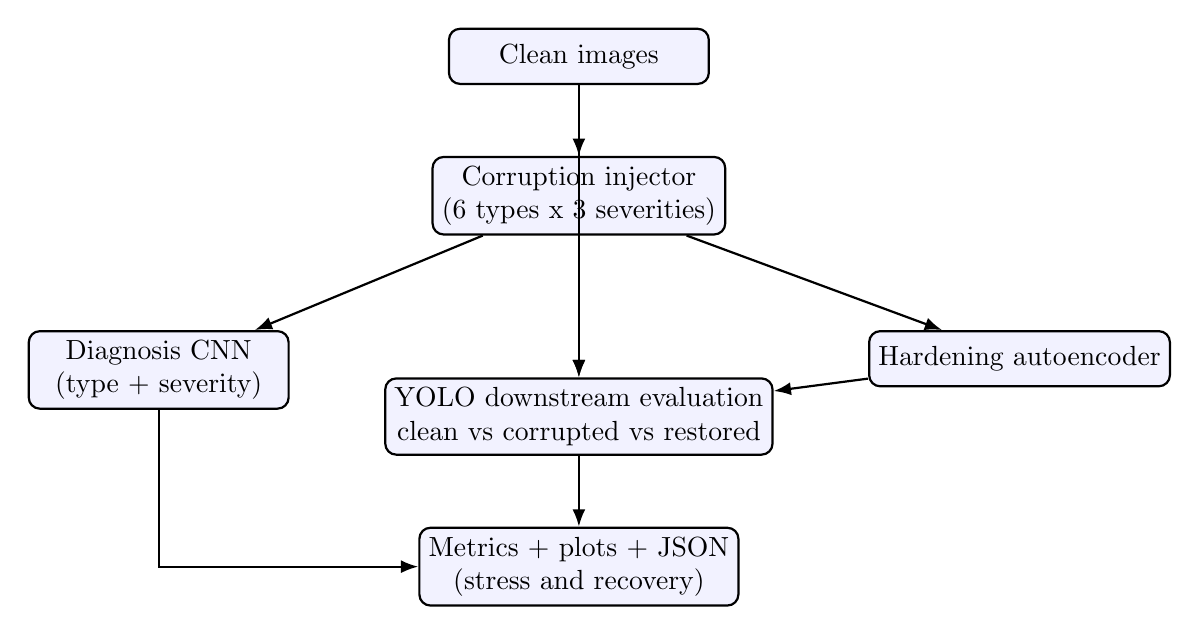
\begin{tikzpicture}[
  node distance=9mm,
  block/.style={rectangle, rounded corners, draw=black, thick, minimum width=33mm, minimum height=7mm, align=center, fill=blue!5},
  line/.style={-{Latex[length=2.2mm]}, thick}
]
\node[block] (clean) {Clean images};
\node[block, below=of clean] (inject) {Corruption injector\\(6 types x 3 severities)};
\node[block, below left=12mm and 18mm of inject] (diag) {Diagnosis CNN\\(type + severity)};
\node[block, below right=12mm and 18mm of inject] (hard) {Hardening autoencoder};
\node[block, below=18mm of inject] (det) {YOLO downstream evaluation\\clean vs corrupted vs restored};
\node[block, below=of det] (sum) {Metrics + plots + JSON\\(stress and recovery)};

\draw[line] (clean) -- (inject);
\draw[line] (inject) -- (diag);
\draw[line] (inject) -- (hard);
\draw[line] (clean) -- (det);
\draw[line] (inject) -- (det);
\draw[line] (hard) -- (det);
\draw[line] (diag) |- (sum);
\draw[line] (det) -- (sum);
\end{tikzpicture}
\caption{End-to-end research pipeline implemented in this project.}
\label{fig:flowchart}
\end{figure}

\subsection{Corruption model}
Let $J(x)$ be the clean image and $I(x)$ be the corrupted observation. The injector implements six corruption families. Example atmospheric haze model:
\begin{equation}
I(x) = J(x)\,t(x) + A\,(1-t(x)), \quad t(x)=e^{-\beta d(x)}
\end{equation}
where $A$ is atmospheric light, $\beta$ controls scattering, and $d(x)$ is spatial depth proxy.

Other implemented corruptions are Gaussian blur, JPEG artifacts, mixed sensor noise, radiometric drift, and spectral band misalignment.

\subsection{Diagnosis network}
A ResNet-based multi-task CNN predicts:
\begin{enumerate}
\item corruption type ($7$ classes including clean),
\item corruption severity ($3$ classes).
\end{enumerate}
The combined loss is:
\begin{equation}
\mathcal{L}_{diag} = w_t\,\mathcal{L}_{CE}(y_t,\hat{y}_t) + w_s\,\mathcal{L}_{CE}(y_s,\hat{y}_s)
\end{equation}

\subsection{Hardening network}
The restoration model is a U-Net-style autoencoder with Kick decoder branches to reduce checkerboard artifacts. The objective is:
\begin{equation}
\mathcal{L}_{hard} = \lambda_1 \mathcal{L}_{L1} + \lambda_2 \mathcal{L}_{perc} + \lambda_3 \mathcal{L}_{SSIM}
\end{equation}

\subsection{Downstream metric and recovery criterion}
Detector outputs are measured on clean, corrupted, and hardened images. Recovery is defined as:
\begin{equation}
\text{Recovery}(\%) = \frac{D_{hard} - D_{corr}}{D_{clean}-D_{corr}} \times 100
\end{equation}
where $D$ denotes average detection count for the corresponding set.

\subsection{Core evaluation algorithm}
\begin{algorithm}[H]
\caption{Corruption-to-Recovery Evaluation}
\begin{algorithmic}[1]
\For{each clean image $x$}
  \State compute clean detector count
\EndFor
\For{corruption type $c \in \{1..6\}$}
  \For{severity $s \in \{0,1,2\}$}
    \For{each clean image $x$}
      \State $x_{corr} \leftarrow \text{Inject}(x,c,s)$
      \State $(\hat{c},\hat{s}) \leftarrow \text{DiagnosisCNN}(x_{corr})$
      \State $x_{hard} \leftarrow \text{Hardener}(x_{corr})$
      \State record PSNR/SSIM between $x$ and $x_{hard}$
      \State record detector counts on $x_{corr}$ and $x_{hard}$
    \EndFor
    \State aggregate diagnosis, quality, and recovery metrics
  \EndFor
\EndFor
\end{algorithmic}
\end{algorithm}

\section{Experimental Setup}
\subsection{Dataset}
EuroSAT folder used in this implementation: $27{,}000$ images, 10 classes, approximately 87.59 MB on disk in this workspace.

\subsection{Training configuration used for demonstrated run}
\begin{table}[H]
\centering
\caption{Demonstration run settings (reproducible quick run)}
\begin{tabular}{ll}
\toprule
Parameter & Value \\
\midrule
Image size & $64 \times 64$ \\
Epochs & 1 \\
Batch size & 4 \\
Max source images & 10 \\
Workers & 0 (Windows-safe) \\
Diagnosis parameters & 11,375,690 \\
Hardener parameters & 61,714,886 \\
\bottomrule
\end{tabular}
\label{tab:setup}
\end{table}

\subsection{Training sample expansion}
For 10 source images:
\begin{itemize}
\item Diagnosis dataset: $10 \times (1 + 6\times3) = 190$ samples (train 152, val 38)
\item Autoencoder dataset: $10 \times 6 = 60$ samples (train 48, val 12)
\end{itemize}

\section{Results}
\subsection{Diagnosis behavior}
From the current evaluation run, diagnosis accuracy is highly corruption-dependent (e.g., blur significantly higher than JPEG and band misalignment).

\begin{table}[H]
\centering
\caption{Diagnosis accuracy by corruption family (from current run)}
\begin{tabular}{lc}
\toprule
Corruption & Accuracy (\%) \\
\midrule
Haze & 26.7 \\
Blur & 86.7 \\
JPEG & 10.0 \\
Noise & 63.3 \\
Radiometric drift & 60.0 \\
Band misalignment & 13.3 \\
\bottomrule
\end{tabular}
\label{tab:diag}
\end{table}

\subsection{Downstream stress and recovery}
The clean baseline is low ($0.30$ average detections/image), so recovery percentages can appear numerically large for small absolute changes. Therefore, recovery should be interpreted jointly with absolute clean/corrupted/hardened counts.

\begin{table}[H]
\centering
\caption{How to interpret key downstream indicators}
\begin{tabular}{p{40mm}p{95mm}}
\toprule
Indicator & Interpretation \\
\midrule
Detection Drop \% & Relative degradation from clean to corrupted input \\
Recovery \% & Relative regain from corrupted to hardened input \\
Recovery $>100\%$ & Hardened output exceeded clean baseline for that slice \\
Recovery $<0\%$ & Hardening worsened downstream behavior for that slice \\
\bottomrule
\end{tabular}
\label{tab:interpret}
\end{table}

\subsection{Qualitative and dashboard outputs}
Upload these generated files to Overleaf and keep names unchanged.

\begin{figure}[H]
\centering
\maybegraphic{outputs/evaluation/dashboard.png}{width=0.95\linewidth}{}
\caption{Evaluation dashboard generated by the implemented pipeline.}
\label{fig:dashboard}
\end{figure}

\begin{figure}[H]
\centering
\maybegraphic{outputs/evaluation/stress_curves.png}{width=0.95\linewidth}{}
\caption{Stress curves: clean vs corrupted vs hardened trends across severity levels.}
\label{fig:stress}
\end{figure}

\begin{figure}[H]
\centering
\begin{subfigure}{0.48\linewidth}
\centering
\maybegraphic{outputs/visualizations/AnnualCrop_1_corruption_grid.png}{width=\linewidth}{}
\caption{Sample A}
\end{subfigure}
\hfill
\begin{subfigure}{0.48\linewidth}
\centering
\maybegraphic{outputs/visualizations/AnnualCrop_10_corruption_grid.png}{width=\linewidth}{}
\caption{Sample B}
\end{subfigure}
\caption{Corruption grids used for qualitative validation of failure simulation.}
\label{fig:corruptions}
\end{figure}

\section{Discussion}
\subsection{What we can conclude confidently}
\begin{enumerate}
\item Preprocessing failures produce measurable and non-uniform downstream degradation.
\item Diagnosis quality varies by corruption family, suggesting feature separability differs by failure type.
\item Restoration can recover performance in some corruption regimes but not uniformly across all regimes.
\item Stress-curve analysis is more informative than a single aggregate score.
\end{enumerate}

\subsection{Threats to validity}
\begin{enumerate}
\item Current demonstrated run uses small training budget (epochs/images) for speed.
\item EuroSAT is not a dedicated detection benchmark; downstream count behavior should be interpreted as robustness trend evidence.
\item Very low clean baseline can inflate relative recovery percentages.
\end{enumerate}

\section{Conclusion}
This work provides an end-to-end, reproducible implementation for studying how preprocessing quality affects machine learning systems in satellite imaging workflows. The framework unifies physically motivated failure simulation, learned diagnosis, learned restoration, and downstream stress testing into one pipeline. Results show that preprocessing robustness is corruption-specific and should be reported as structured stress/recovery behavior rather than clean-set accuracy alone.

\section*{Reproducibility Appendix (commands)}
\begin{verbatim}
python main.py --mode full_pipeline \
  --image_dir ./datasets/eurosat/eurosat/2750 \
  --image_size 64 --epochs 1 --batch_size 4 --max_images 10 --num_workers 0
\end{verbatim}

\begin{thebibliography}{9}
\bibitem{prathyusha2025yolo}
G. Prathyusha, K. Deekshitha Reddy, K. Harshitha, and L. Rajasri,
"YOLOv8-Based Detection System for Military Vehicle Recognition in Satellite Imagery,"
in \emph{Proc. 6th Int. Conf. Inventive Research in Computing Applications (ICIRCA)}, 2025, pp. 815--821, doi: 10.1109/ICIRCA65293.2025.11089616.

\bibitem{sensors2022landsat}
A. F. M. S. et al.,
"A Single Image Deep Learning Approach to Restoration of Corrupted Landsat-7 Satellite Images,"
\emph{Sensors}, vol. 22, no. 23, 9273, 2022.

\bibitem{ultralytics}
G. Jocher et al.,
"Ultralytics YOLOv8," \url{https://github.com/ultralytics/ultralytics}, accessed 2026.
\end{thebibliography}

\end{document}
